\section{Ajuste por mínimos cuadrados}

\subsection{Hipótesis}

Para verificar que el tiempo de ejecución del algoritmo es $O(n \log n)$, realizamos un ajuste por mínimos cuadrados. La función que queremos ajustar es de la forma:
\[f(n) = a \cdot n \log n + b\]
donde $a$ y $b$ son los parámetros a ajustar.

\subsection{Datos de entrada}

Los datos de entrada para el ajuste son los siguientes:

\begin{itemize}
    \item $n$: Tamaño del problema (número de batallas).
    \item $T(n)$: Tiempo de ejecución medido para cada tamaño $n$.
\end{itemize}

\subsection{Recopilación de datos}

Para obtener mediciones confiables y reducir el ruido, seguimos los siguientes pasos:

\begin{itemize}
    \item \textbf{Múltiples tamaños:} Probamos con $n = 1000, 2000, 4000, 8000, 16000, 32000, 50000$.
    \item \textbf{Múltiples datasets:} Para cada tamaño $n$, generamos 8 conjuntos de datos diferentes.
    \item \textbf{Múltiples repeticiones:} Cada dataset se ejecuta varias veces.
    \item \textbf{Filtrado de outliers:} Eliminamos mediciones extremas y promediamos.
\end{itemize}

\subsection{Codigo utilizado}

\begin{lstlisting}[language=Python, caption=Código para ajuste por mínimos cuadrados]
import numpy as np
import matplotlib.pyplot as plt
import time
import random

from tp1 import orden_batallas

def generar_datos_aleatorios(n, seed=1234):
    random.seed(seed)
    batallas = []
    for _ in range(n):
        t_i = random.randint(1, 1000)
        b_i = random.randint(1, 1000)
        batallas.append([t_i, b_i])
    return batallas

def medir_tiempo(batallas, repeticiones=10):
    tiempos = []
    for _ in range(repeticiones):
        batallas_copia = [batalla.copy() for batalla in batallas]
        inicio = time.perf_counter()
        orden_batallas(batallas_copia)
        fin = time.perf_counter()
        tiempos.append(fin - inicio)
    
    # Eliminar outliers (20% superior e inferior)
    tiempos_ordenados = sorted(tiempos)
    n_mediciones = len(tiempos_ordenados)
    inicio_idx = int(n_mediciones * 0.2)
    fin_idx = int(n_mediciones * 0.8)
    tiempos_filtrados = tiempos_ordenados[inicio_idx:fin_idx]
    
    return np.mean(tiempos_filtrados)

# ==================== PASO 1: Recoleccion de datos ==================== #

def recolectar_datos():
    print("=== PASO 1: RECOLECCION DE DATOS ===")
    tamanos = [500, 1000, 2000, 4000, 8000, 16000, 32000, 64000, 128000, 256000, 512000, 1024000, 2048000]
    
    cantidades = []
    tiempos = []
    
    print("Midiendo tiempos...")
    for n in tamanos:
        print(f"  Midiendo n = {n}...")
        
        # Generar multiples datasets y promediar
        tiempos_n = []
        for seed in range(5):  # 5 datasets diferentes
            datos = generar_datos_aleatorios(n, seed + 42)
            tiempo = medir_tiempo(datos, repeticiones=8)
            tiempos_n.append(tiempo)
        
        tiempo_promedio = np.mean(tiempos_n)
        
        cantidades.append(n)
        tiempos.append(tiempo_promedio * 1000)  # Convertir a milisegundos
        
        print(f"    Tiempo promedio: {tiempo_promedio * 1000:.3f} ms")
    
    return cantidades, tiempos

# ==================== PASO 2: Ajuste por cuadrados minimos ==================== #

def ajuste_nlogn(cantidades, tiempos):
    print("\n=== PASO 2: AJUSTE POR CUADRADOS MINIMOS PARA O(n log n) ===")
    
    # Convertir a arrays de numpy
    cantidades = np.array(cantidades)
    tiempos = np.array(tiempos)
    
    x = cantidades * np.log(cantidades)

    A = np.vstack([x, np.ones(len(x))]).T

    AtA = np.dot(A.T, A)
    Atb = np.dot(A.T, tiempos)
    coeficientes = np.linalg.solve(AtA, Atb)
    b, a = coeficientes  # b es la pendiente, a es la ordenada al origen
    
    tiempos_predichos = a + b * x
    errores_residuales = tiempos - tiempos_predichos

    ss_res = np.sum(errores_residuales**2)
    ss_tot = np.sum((tiempos - np.mean(tiempos))**2)
    r_cuadrado = 1 - (ss_res / ss_tot)

    return a, b, r_cuadrado, x, tiempos_predichos, errores_residuales

# ==================== PASO 3: Graficos de verificacion ==================== #

def generar_grafico_verificacion(cantidades, tiempos, a, b, r_cuadrado, x_modelo, t_predicho):
    print("\n=== GENERANDO GRAFICO DE VERIFICACION ===")
    
    # Configurar el grafico
    plt.figure(figsize=(12, 8))
    
    # ==================== PUNTOS MEDIDOS ==================== #
    plt.scatter(x_modelo, tiempos, color='blue', s=100, alpha=0.8, 
                label='Tiempos medidos', zorder=5, edgecolors='darkblue', linewidth=1)
    
    # ==================== FUNCION ESTIMADA ==================== #
    # Crear una curva suave para la funcion estimada
    n_smooth = np.linspace(min(cantidades), max(cantidades), 200)
    x_smooth = n_smooth * np.log2(n_smooth)
    t_smooth = a + b * x_smooth
    
    plt.plot(x_smooth, t_smooth, color='red', linewidth=3, 
             label=f'Funcion estimada: T(n) = {a:.3f} + {b:.6f}x(n log n)')
    
    # ==================== CONFIGURACION DEL GRAFICO ==================== #
    plt.xlabel('n x log(n)', fontsize=14, fontweight='bold')
    plt.ylabel('Tiempo de ejecucion (ms)', fontsize=14, fontweight='bold')
    plt.title(f'Verificacion de Complejidad O(n log n)\nR^2 = {r_cuadrado:.6f}', 
              fontsize=16, fontweight='bold', pad=20)
    
    plt.grid(True, alpha=0.3, linestyle='--')
    plt.legend(fontsize=12, framealpha=0.9)
    
    # ==================== CAJA DE INFORMACION ==================== #
    info_text = f"""METODO DE CUADRADOS MINIMOS
    
- Hipotesis: T(n) ~ n x log(n)
- Modelo ajustado: T(n) = a + b (n log(n))
- Coeficiente R^2 = {r_cuadrado:.6f}
"""
    
    plt.text(0.02, 0.98, info_text, transform=plt.gca().transAxes, 
             fontsize=11, verticalalignment='top',
             bbox=dict(boxstyle="round,pad=0.5", facecolor="lightyellow", alpha=0.9))
    
    # ==================== INTERPRETACION ==================== #
    if r_cuadrado > 0.98:
        conclusion = "COMPLEJIDAD O(n log n) VERIFICADA"
        color_conclusion = "lightgreen"
    elif r_cuadrado > 0.95:
        conclusion = "Complejidad O(n log n) muy probable"
        color_conclusion = "lightblue"
    else:
        conclusion = "Resultados no concluyentes"
        color_conclusion = "lightyellow"
    
    plt.text(0.98, 0.02, conclusion, transform=plt.gca().transAxes, 
             fontsize=12, fontweight='bold', horizontalalignment='right',
             bbox=dict(boxstyle="round,pad=0.5", facecolor=color_conclusion, alpha=0.9))
    
    # ==================== LINEAS DE ERROR ==================== #
    # Mostrar las diferencias entre puntos medidos y predichos
    for i in range(len(x_modelo)):
        plt.plot([x_modelo[i], x_modelo[i]], [tiempos[i], t_predicho[i]], 
                'gray', linestyle=':', alpha=0.6, linewidth=1)
    
    plt.tight_layout()
    plt.savefig('verificacion_complejidad_nlogn.png', dpi=300, bbox_inches='tight')
    plt.show()

# ==================== FUNCION PRINCIPAL ==================== #
def main():
    print("[VERIFICACION DE COMPLEJIDAD O(n log n)]")
    print("Algoritmo: Ordenamiento de batallas por ratio b/t")
    print("Metodo: Cuadrados minimos con ajuste lineal\n")
    
    # Ejecutar todos los pasos
    cantidades, tiempos = recolectar_datos()
    a, b, r_cuadrado, x, y_predicho, _ = ajuste_nlogn(cantidades, tiempos)
    generar_grafico_verificacion(cantidades, tiempos, a, b, r_cuadrado, x, y_predicho)

    print("\nAnalisis completado.")
    print(f"Resultados del ajuste: a = {a:.6f}, b = {b:.6f}, R^2 = {r_cuadrado:.6f}")
    print("Conclusion: La complejidad del algoritmo es O(n log n) debido a la alta calidad del ajuste.")

if __name__ == "__main__":
    main()
\end{lstlisting}

\subsection{Resultados del ajuste}

Los resultados del ajuste por mínimos cuadrados son:

\begin{itemize}
    \item Coeficientes ajustados: $a = -3.078542$, $b = 0.000051$
    \item Calidad del ajuste: $R^2 = 0.999912$
    \end{itemize}

\begin{figure}[H]
    \centering
    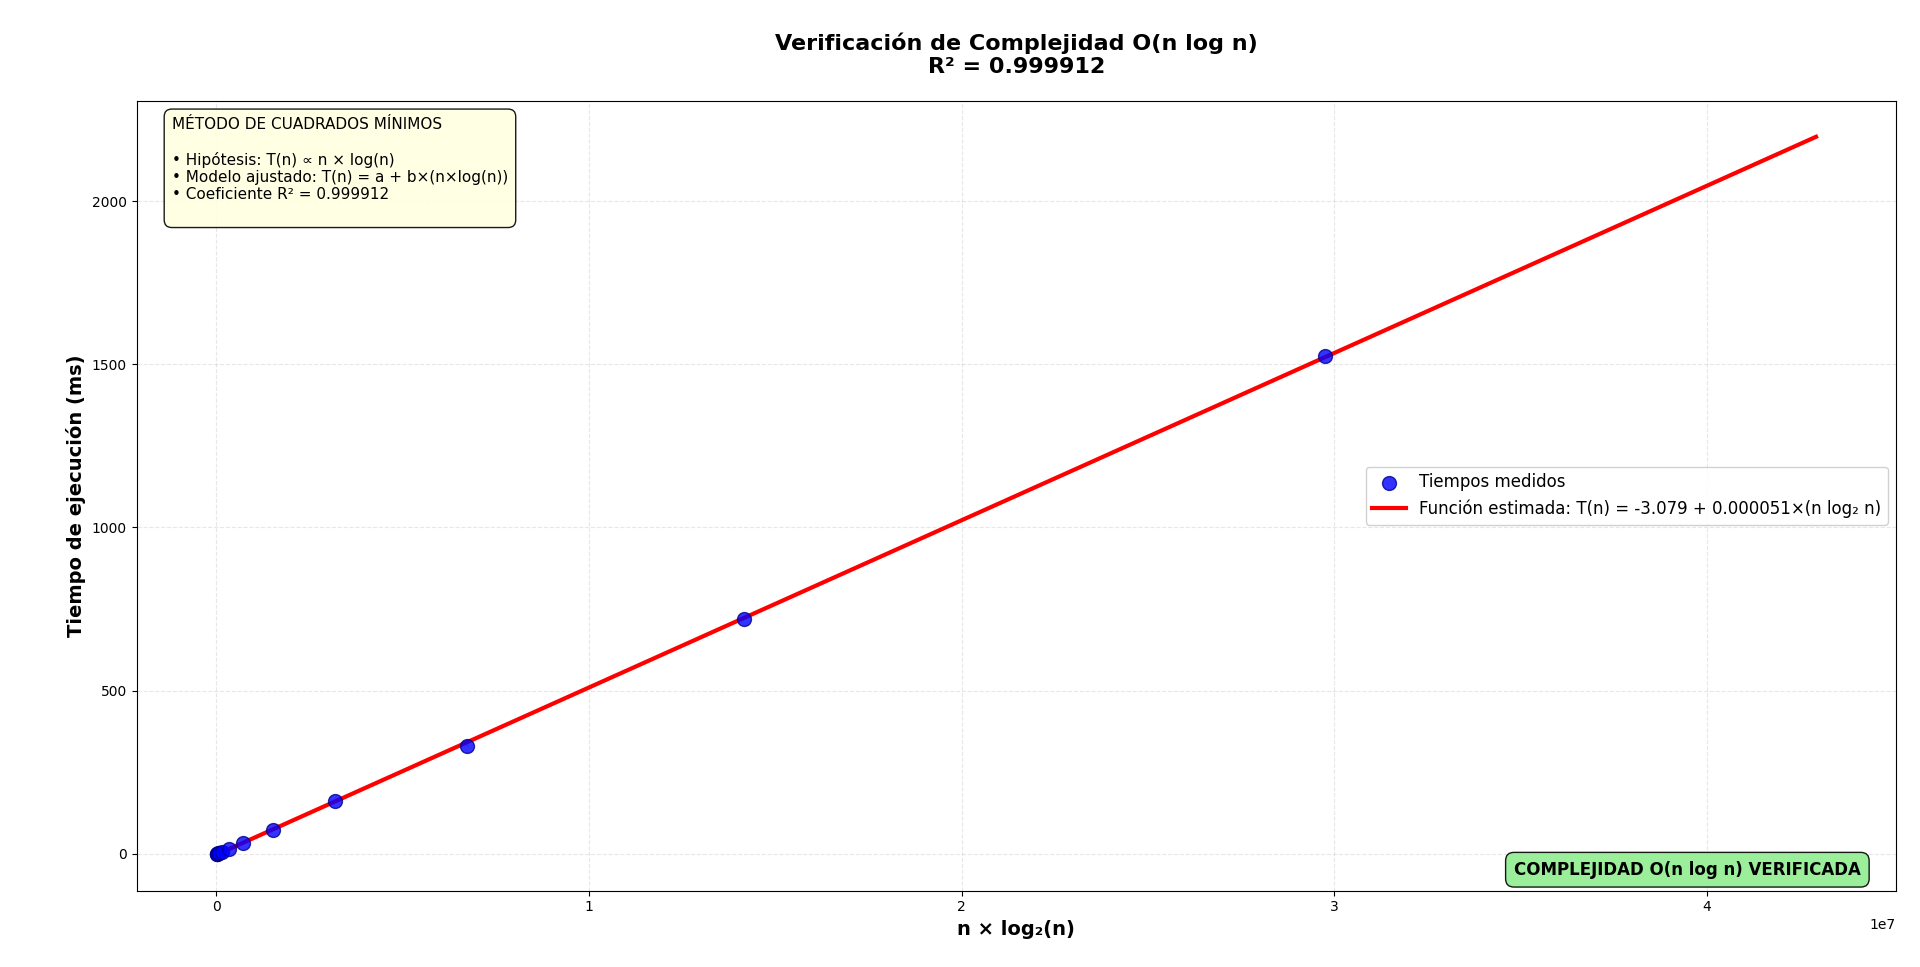
\includegraphics[width=0.8\textwidth]{./img/Figure_1.png}
    \caption{Gráfico de verificación de complejidad $O(n \log n)$}
\end{figure}

\subsection{Interpretacion de resultados}

Usamos el coeficiente de determinacion R²:

\begin{itemize}
    \item $R^2$ = 1.00: Ajuste perfecto (0\% de error)
    \item $R^2$ mayor 0.98: Excelente ajuste → Complejidad verificada
    \item $R^2$ mayor 0.95: Muy buen ajuste → Complejidad muy probable
    \item $R^2$ menor 0.90: Ajuste pobre → Resultados no concluyentes
\end{itemize}

\subsection{Conclusion}

Con un valor de $R^2 = 0.999912$, concluimos que la complejidad del algoritmo es $O(n \log n)$ debido a la alta calidad del ajuste.